% Options for packages loaded elsewhere
\PassOptionsToPackage{unicode}{hyperref}
\PassOptionsToPackage{hyphens}{url}
%
\documentclass[
]{article}
\usepackage{amsmath,amssymb}
\usepackage{iftex}
\ifPDFTeX
  \usepackage[T1]{fontenc}
  \usepackage[utf8]{inputenc}
  \usepackage{textcomp} % provide euro and other symbols
\else % if luatex or xetex
  \usepackage{unicode-math} % this also loads fontspec
  \defaultfontfeatures{Scale=MatchLowercase}
  \defaultfontfeatures[\rmfamily]{Ligatures=TeX,Scale=1}
\fi
\usepackage{lmodern}
\ifPDFTeX\else
  % xetex/luatex font selection
\fi
% Use upquote if available, for straight quotes in verbatim environments
\IfFileExists{upquote.sty}{\usepackage{upquote}}{}
\IfFileExists{microtype.sty}{% use microtype if available
  \usepackage[]{microtype}
  \UseMicrotypeSet[protrusion]{basicmath} % disable protrusion for tt fonts
}{}
\makeatletter
\@ifundefined{KOMAClassName}{% if non-KOMA class
  \IfFileExists{parskip.sty}{%
    \usepackage{parskip}
  }{% else
    \setlength{\parindent}{0pt}
    \setlength{\parskip}{6pt plus 2pt minus 1pt}}
}{% if KOMA class
  \KOMAoptions{parskip=half}}
\makeatother
\usepackage{xcolor}
\usepackage[margin=1in]{geometry}
\usepackage{graphicx}
\makeatletter
\def\maxwidth{\ifdim\Gin@nat@width>\linewidth\linewidth\else\Gin@nat@width\fi}
\def\maxheight{\ifdim\Gin@nat@height>\textheight\textheight\else\Gin@nat@height\fi}
\makeatother
% Scale images if necessary, so that they will not overflow the page
% margins by default, and it is still possible to overwrite the defaults
% using explicit options in \includegraphics[width, height, ...]{}
\setkeys{Gin}{width=\maxwidth,height=\maxheight,keepaspectratio}
% Set default figure placement to htbp
\makeatletter
\def\fps@figure{htbp}
\makeatother
\setlength{\emergencystretch}{3em} % prevent overfull lines
\providecommand{\tightlist}{%
  \setlength{\itemsep}{0pt}\setlength{\parskip}{0pt}}
\setcounter{secnumdepth}{-\maxdimen} % remove section numbering
\ifLuaTeX
  \usepackage{selnolig}  % disable illegal ligatures
\fi
\IfFileExists{bookmark.sty}{\usepackage{bookmark}}{\usepackage{hyperref}}
\IfFileExists{xurl.sty}{\usepackage{xurl}}{} % add URL line breaks if available
\urlstyle{same}
\hypersetup{
  pdftitle={SUFRAGISMO},
  pdfauthor={Tomàs Ferrandis Moscardó},
  hidelinks,
  pdfcreator={LaTeX via pandoc}}

\title{SUFRAGISMO}
\author{Tomàs Ferrandis Moscardó}
\date{2022-11-23}

\begin{document}
\maketitle

{
\setcounter{tocdepth}{2}
\tableofcontents
}
A cierta edad, al volver a estudiar Historia Contemporánea te encuentras
protagonistas que en tu juventud quedaron fuera de los libros de texto.
Impresiona ver hasta qué punto se ha tergiversado u ocultado el papel de
la mujer. Comenta un compañero que la misma imagen de la Revolución
Industrial, por ejemplo, es la de un obrero varón. ¿Acaso no trabajaban
hasta los niños?, ¿quién, tras la interminable jornada laboral tenía una
``segunda jornada''? Por no hablar de la iniciativa y el gran papel de
las mujeres en las revoluciones o su aportación silenciada en tantos
campos del conocimiento.

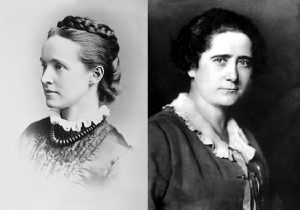
\includegraphics{png/Clara_Campoamor-y-Millicent_Garret.jpg}

\emph{Foto: Millicent Garrett ( 1847-1929). Izq. y Clara Campoamor
(1888-1972). Der.}

Recuerdo, por ejemplo, cómo aprendí el concepto de sufragio universal
frente al sufragio censitario en mi niñez. Aquel ``universal'' sin más
dejaba fuera a medio universo; se consiguió el sufragio universal y lo
de la mujer vino después, como remate a la faena.

Tras despertarse en mi el interés por el sufragismo me decidí por la
lectura de dos libros autobiográficos como forma de rescatar mujeres del
silencio de historia: ``El voto femenino y yo. Mi pecado mortal'' de
Clara Campoamor y ``Sufragio femenino. Breve historia de un gran
movimiento'' de Millicent Garrett, menos conocido. Pese a la diferencia
de casi medio siglo entre ambas sufragistas y la diferencia de años en
la legalización del voto femenino en España e Inglaterra, los dos
testimonios coinciden en muchos aspectos desdibujando la imagen que
tenemos del sufragismo. Veamos.

\hypertarget{sufragismo-muxe1s-alluxe1-del-voto-de-la-mujer}{%
\subsection{Sufragismo, más allá del voto de la
mujer}\label{sufragismo-muxe1s-alluxe1-del-voto-de-la-mujer}}

El sufragismo se nos presenta habitualmente como una lucha con un
objetivo único, una reivindicación aislada por un derecho fundamental de
las mujeres y que se libró en los países occidentales. En este sentido
siempre se destacan las sufragistas inglesas presididas por Emmili
Pankhurst en la Inglaterra del siglo XIX o en el caso español, las
diputadas Clara Campoamor y Victoria Kent en su batalla por el sufragio
pasivo femenino en la España de la 2ª República.

\hypertarget{otras-causas-de-la-mujer}{%
\subsubsection{Otras causas de la
mujer}\label{otras-causas-de-la-mujer}}

Millicent Garrett en sus memorias (Garret, 2020) explica cómo, si bien
las sociedades sufragistas se centraban en el voto femenino, a nivel
individual, las principales militantes consiguieron mejorar el estado
legal de las mujeres con ``resultados inesperados'' en la década de 1830
consiguiendo una ley de propiedades de la mujer casada, una ley de
custodia de menores, el derecho al acceso a estudios universitarios, la
mejora de las condiciones laborales discriminatorias de la mujer o el
derecho a ejercer la profesión médica.

Merece nuestra atención la defensa de la abolición de la prostitución y
el combate contra leyes denigrantes hacia las prostitutas de sufragistas
como Josephine Butler.

En la misma línea, casi un siglo después en España, podemos comprobar
que el ideario de Clara Campoamor contemplaba en la década de 1930, como
resume Blanca Estrella (Campoamor, 2006) además del voto femenino, la
ley del divorcio, la ley del derecho del niño y la niña o la ley de
investigación de paternidad.

La misma Campoamor llevará adelante la iniciativa de un Real Decreto
aboliendo la prostitución en la Segunda República y que se llegó a
aprobar gracias a su empeño.

Es evidente que el sufragismo, o al menos, las sufragistas más
destacadas no tenían una única causa por la que luchar.

\hypertarget{cosmovisiuxf3n}{%
\subsection{Cosmovisión}\label{cosmovisiuxf3n}}

Además, como una segunda objeción a una visión reduccionista del
sufragismo debemos recabar que, el sufragismo inglés del XIX y el
español del siglo XX, tenían una mirada sobre los problemas sociales que
alcanzaba más allá de su mundo, de los problemas que afectaban a las
mujeres de su sociedad. De nuevo podremos establecer paralelismos si
tomamos nota de la lucha contra el esclavismo en EEUU y el pacifismo
antibelicista de aquellas sufragistas inglesas y la lucha contra la pena
de muerte de Campoamor y sus propuestas a las Cortes Generales a favor
del desarme declarándose ``pacifista hasta la intransigencia''.

En definitiva, el pacifismo y el abolicionismo como respuesta a toda
denigración del ser humano (esclavitud o prostitución) entran en el
ideario sufragista o en su visión de la dignidad humana y modelo liberal
o republicano de sociedad.

\begin{figure}
\centering
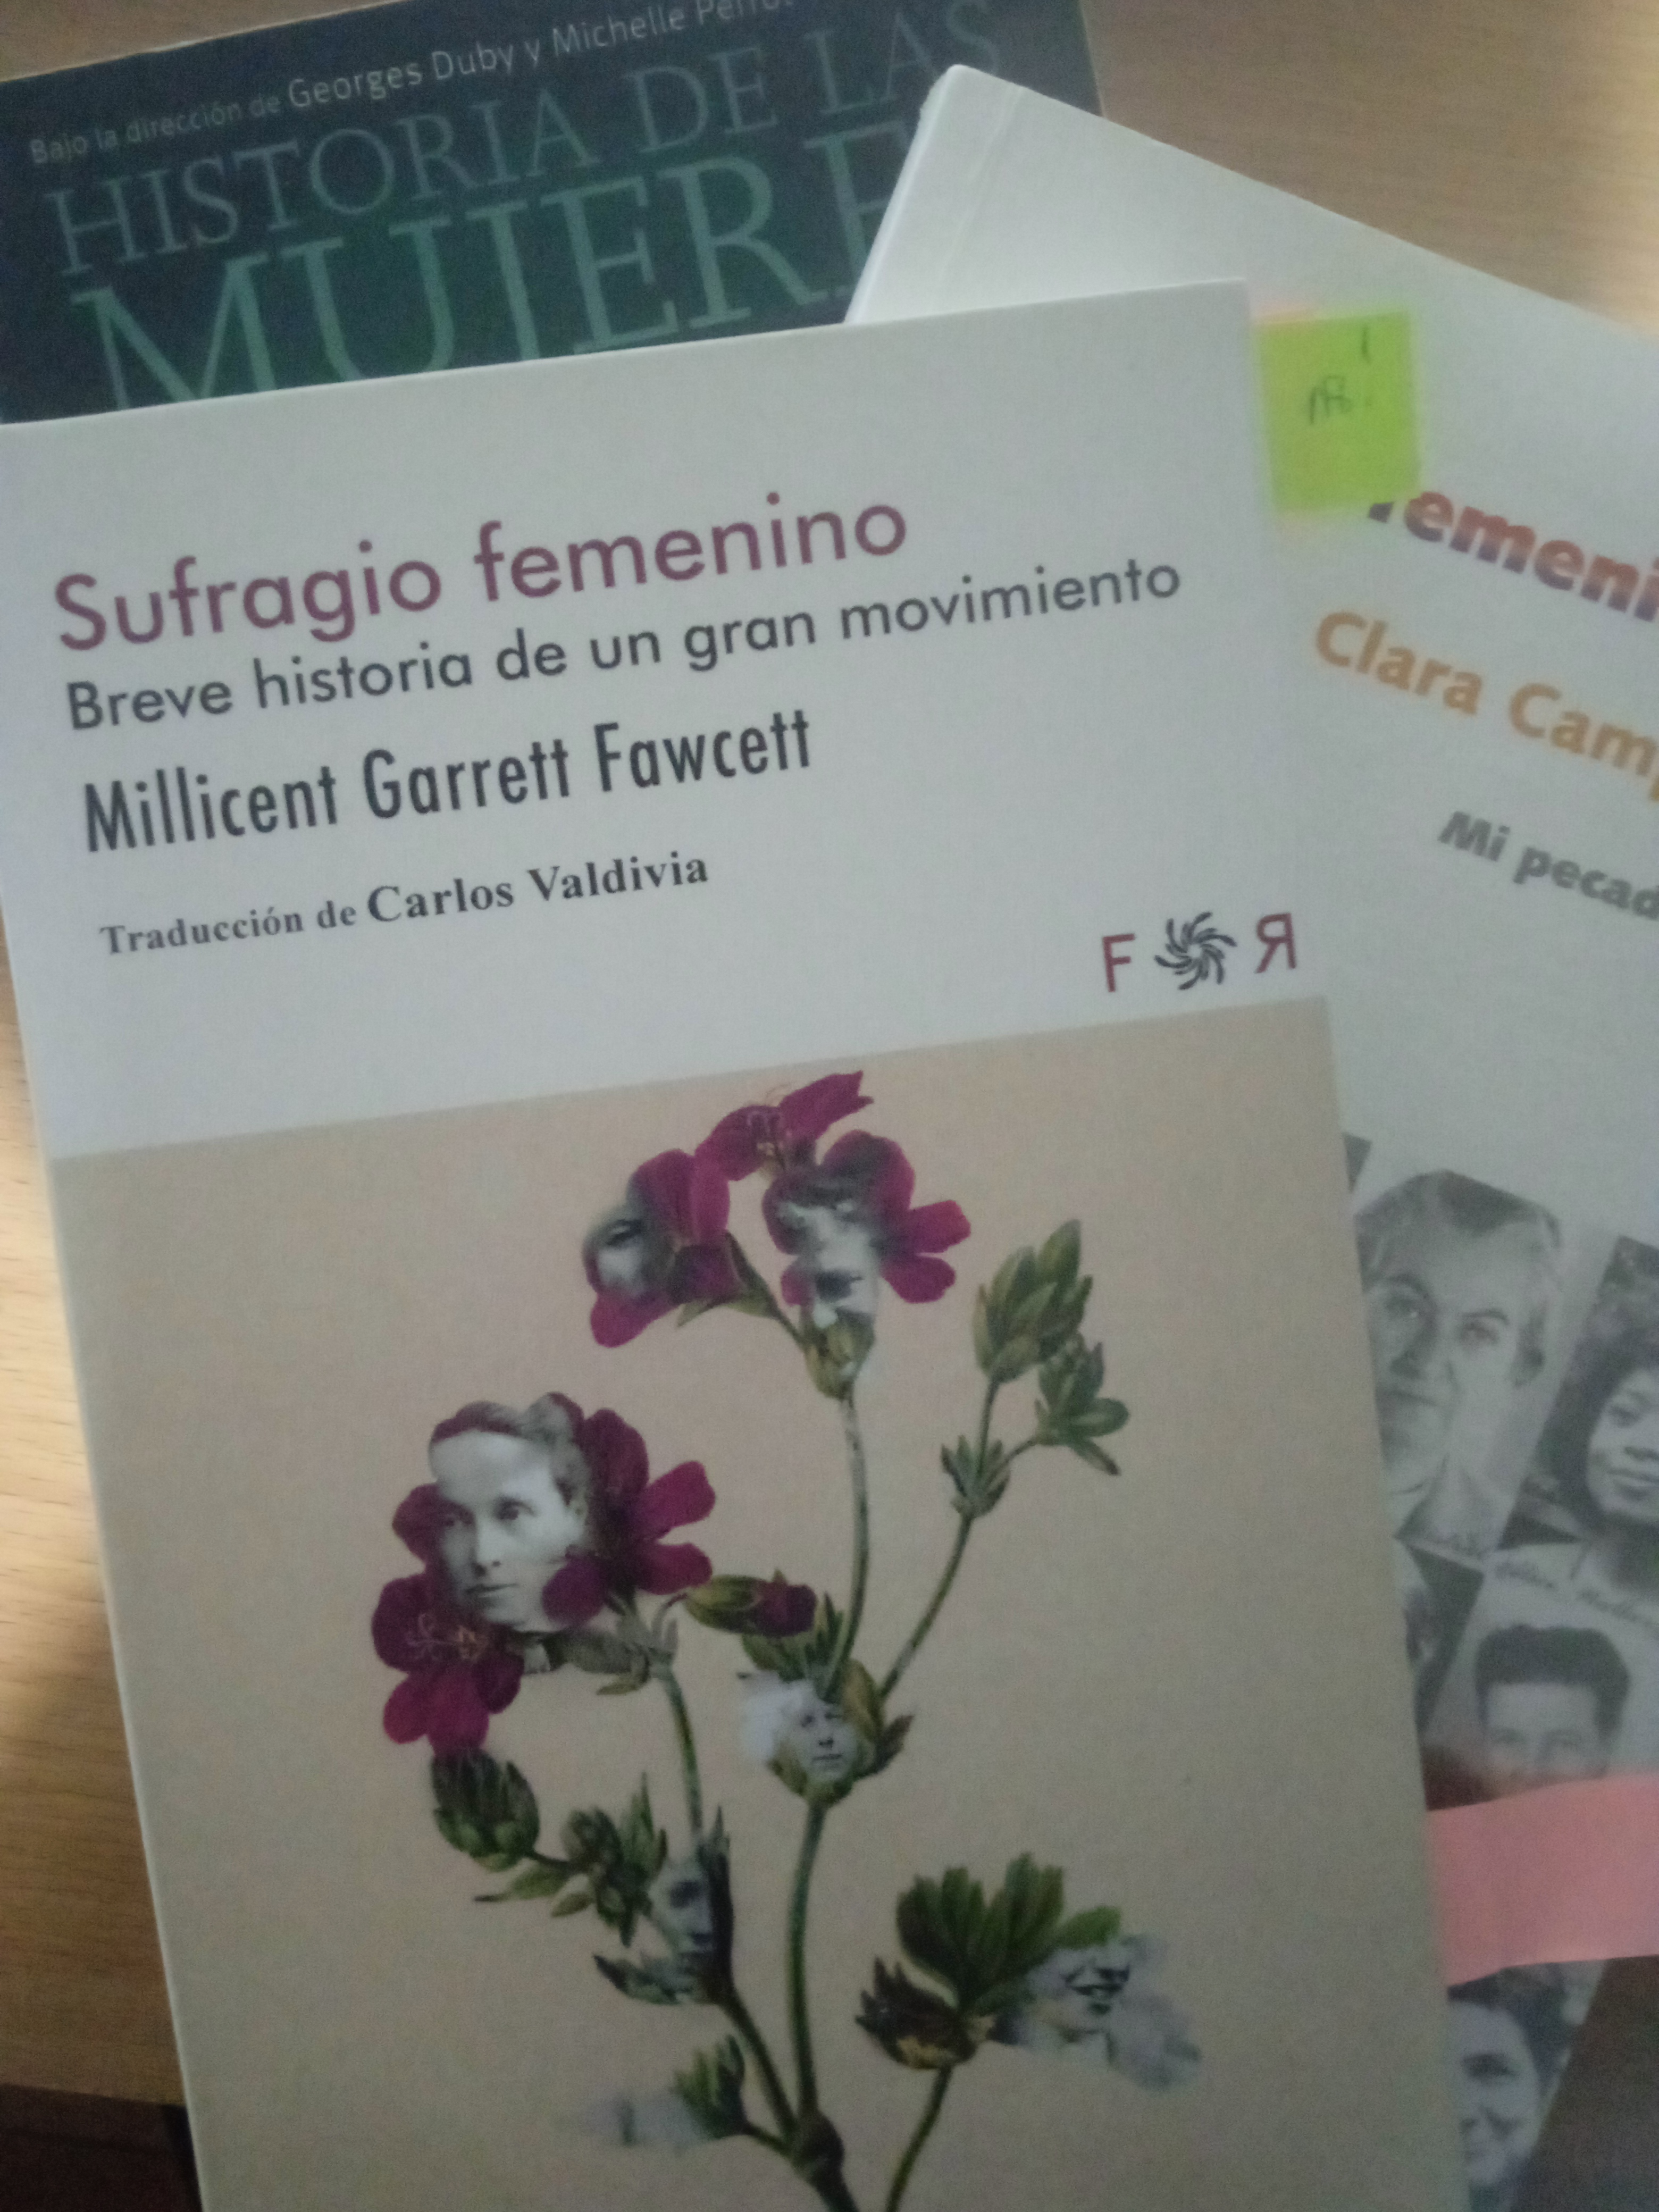
\includegraphics[width=3.125in,height=\textheight]{png/Fuentes.jpg}
\caption{Foto: Bibliografía}
\end{figure}

\hypertarget{el-voto-como-instrumento}{%
\subsubsection{El voto como
instrumento}\label{el-voto-como-instrumento}}

A la visión sesgada del sufragismo como lucha por el voto de la mujer
cabe hacer otra objeción. Si bien el sufragismo reclama el derecho como
principio de igualdad es, precisamente, porque lo entiende como una
condición imprescindible para conseguir la igualdad en derechos privados
y públicos entre hombre y mujer. No se trata de la exigencia de un
derecho sino de un empoderamiento con fin instrumental para poder
avanzar hacia la plena igualdad.

\hypertarget{el-sufragio-no-vino-de-la-noche-a-la-mauxf1ana}{%
\subsection{El sufragio no vino de la noche a la
mañana}\label{el-sufragio-no-vino-de-la-noche-a-la-mauxf1ana}}

La batalla por el sufragio femenino es, quizás, uno de los ejemplos más
típicamente usados cuando queremos aleccionar sobre la relación causal
entre ``reivindicación tenaz'' y ``obtención de derechos'': gracias a la
constancia en la protesta se consiguió el voto de la mujer. Solo la
trenacidad acabó por torcer el brazo de parlamentos masculinos. Ni tan
sencillo, ni tan simple.

\hypertarget{uxe9xitos-parciales}{%
\subsubsection{Éxitos parciales}\label{uxe9xitos-parciales}}

El sufragismo llega a su objetivo de voto parlamentario y derecho a ser
parlamentario tras un rosario de éxitos parciales. Éxitos que, desde mi
punto de vista, pueden verse bajo dos prismas:

Son éxitos en sí desde el momento que suponen cambios legales o sociales
que permiten a las mujeres ejercer un derecho que hasta el momento
tenían vetado. Pero son éxitos, además, porqué se abre un campo de
oportunidades o fortalezas para poder influir más en el poder
legislativo, en los partidos políticos o en la sociedad en aras de
conseguir otros objetivos más ambiciosos y, finalemente, el principal de
igualdad en derechos políticos.

Haciendo repaso de estos éxitos tenemos, en primer lugar, el voto y
participación en los consejos escolares de Inglaterra a partir de 1870.
Una situación nueva que permitió ampliar la base del movimiento
sufragista llegando a más mujeres (y hombres).

Un segundo logro fue la legalización del voto femenino en las elecciones
locales, avance que acallaría la voz del antisufragismo. Respecto a este
punto es interesante el testimonio de Garrett, según el cual, donde se
votaba en elecciones municipales cesaban las protestas en contra del
voto femenino al parlamento. Es decir, se desmontaba el argumento
tremendista a medida que se normalizaba el voto femenino.

Un tercer éxito parcial fue la participación de voluntarias en las
campañas electorales de conservadores y liberales (la Prime Rose y la
Federación de mujeres liberales respectivamente) a partir de la
prohibición a los partidos de contratar personal para campañas (Ley de
Reforma 1884 y la Ley de Prácticas Corruptas 1883). Esto facilitó la
influencia de la mujer sobre los partidos y, así, en 1892 se presentó al
parlamento inglés (aunque sin éxito) el primer Proyecto de Ley de
Sufragio Femenino.

Se avanzaba paso a paso. En palabras de Garrett: ``las mujeres de Nueva
Zelanda no se despertaron una buena mañana de 1893, como se ha dicho en
ciertas ocasiones, y se vieron emancipadas''. Y es que no solo influían
los logros que se iban sumando en Inglaterra (o España): hay vida tras
el muro del eurocentrismo que todo lo esconde. También el derecho
reconocido en otros países (incluso entidades subestatales como la Isla
de Man), algunos estados de los EEUU, países del norte de Europa y
especialmente en Nueva Zelanda y Australia (dentro del Imperio
Británico) fueron decisivos para, al menos, romper el argumento del
miedo a ese ``experimento'' que era como denominaban los antisufragistas
al voto femenino.

\hypertarget{causas-y-uxe9xitos.-las-condiciones-de-la-lucha}{%
\subsubsection{Causas y éxitos. Las condiciones de la
lucha}\label{causas-y-uxe9xitos.-las-condiciones-de-la-lucha}}

Anteriormente he reseñado algunas de las causas que abrazaba el
sufragismo. Fuera interesante diferenciar entre ellas, las causas más
universales como el pacifismo, antibelicismo, el abolicionismo de la
esclavitud, de la prostitución por una parte y, en otro apartado
aquellos objetivos o idearios que afectaban de forma particular al
conjunto de las mujeres en su época, sobre todo, el marco legal.

La trifulca entre antisufragismo y sufragismo no representaba una
división más en el debate parlamentario, un acalorado debate similar al
concerniente al impuesto sobre los cereales. El desacuerdo era una
contienda que se libraba de forma muy cruda más allá de las paredes de
Westminster; en la calle, en la fábrica y también en el hogar. Un nuevo
marco jurídico para la relación familiar especialmente asegurando la
custodia de los hijos y el posible divorcio facilitaba, o al menos
dejaba de impedir, la militancia en el sufragismo sin miedo a terribles
represalias. Este es un tema que queda magníficamente retratado en la
película de la directora Sarah Gavron \emph{Suffratte} (2015), traducida
como \emph{Sufragistas}.

\begin{figure}
\centering
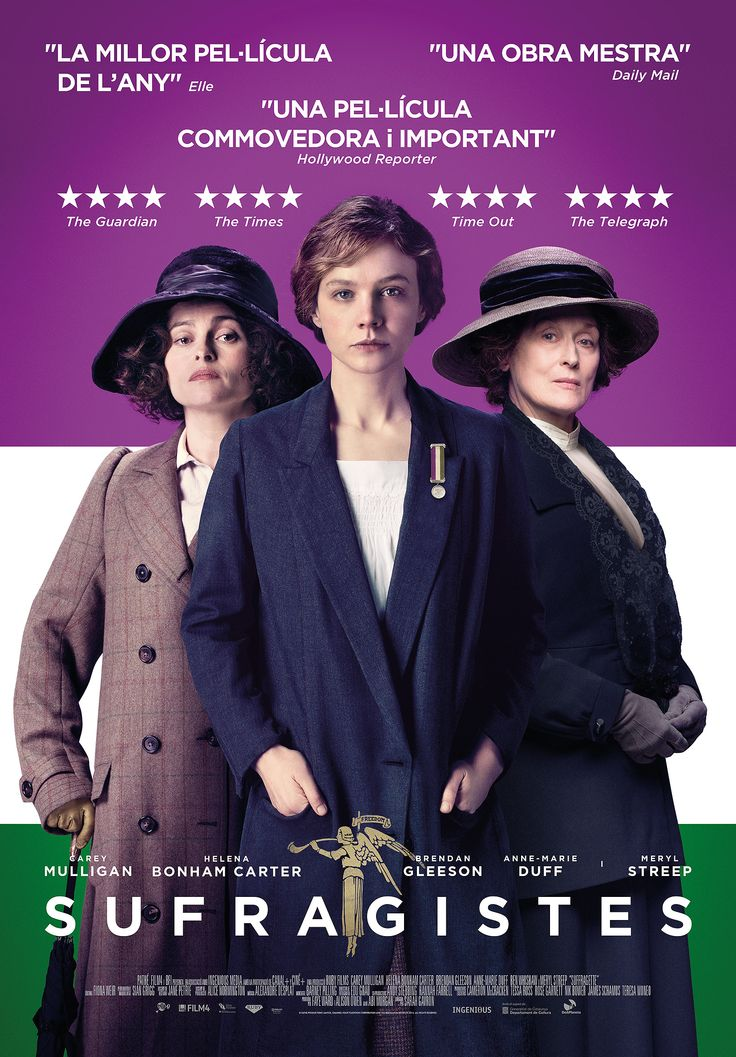
\includegraphics[width=3.125in,height=\textheight]{png/Sufragistes.jpg}
\caption{Foto: Film \emph{Sufragistas}}
\end{figure}

\hypertarget{coincidencias-y-contradicciones}{%
\subsubsection{Coincidencias y
contradicciones}\label{coincidencias-y-contradicciones}}

Como una tercera consideración podríamos hablar de las coincidencias y
alguna peculiaridad de los argumentos de unos y otros, sufragistas y
contrarios al derecho al voto femenino en estas dos épocas y países en
que vivieron Campoamor y Garrett.

\hypertarget{calidad-democruxe1tica}{%
\paragraph{Calidad democrática}\label{calidad-democruxe1tica}}

La correspondencia publicada de John Stuart Mill muestra su preocupación
por la injusticia que supone negar el voto a la mujer, pero también,
como recuerda Millicent Garrett, su clara convicción de que era la
sociedad entera la que salía perjudicada al negarse la responsabilidad
de tratar asuntos nacionales. Es decir, a la razón ética o deseo de
igualdad se sumaba una convicción de que, contando con toda la
población, se iba a mejorar la eficacia o calidad del sistema
democrático.

Clara Campoamor, por su parte, ``consideraba fatal para el resurgimiento
de la libertad y la justicia que veía en la República, el divorcio
espiritual entre hombres y mujeres'' en lo que ella mismo aclaró como su
``pensamiento político y nacional, más amplio y objetivo que el concreto
feminista''.

Por definición el sufragismo es una lucha para que todos los ciudadanos
puedan ejercer los mismos derechos sin distinción de sexo, un
posicionamiento sobre lo que entendemos como derechos fundamentales.
Pero es aquí donde vemos coincidir a Campoamor i Stuart Mill en una
definición más política que defiende una reforma para mejorar el
sistema, el objetivo es la calidad de un buen gobierno, ya no conceder
derechos a ciudadanos.

\hypertarget{el-absurdo-del-antisufragismo}{%
\paragraph{El absurdo del
antisufragismo}\label{el-absurdo-del-antisufragismo}}

Visto hoy en día, llama la atención cómo en la República Española se
discutía en las Cortes Generales con mujeres parlamentarias,
beneficiarias del sufragio pasivo, sobre el derecho de la mujer al
sufragio activo. Cierto es que esta situación, que se nos podría antojar
surrealista, como tal, no se produjo en Inglaterra pero se puede
comparar a otras bien pintorescas que sí se dieron.

Unas décadas antes, las representantes municipales londinenses
integraban las mesas electorales de las elecciones al parlamento en las
que no podían votar. Otro ejemplo sería el de la participación
organizada por los partidos en campañas electorales: las mismas
organizaciones que no las consideraban capacitadas para entender las
complejas razones de la política estatal y votar, las consideraba
preparadas para explicarlas a hombres estas razones y que votasen.
Verdaderamente absurdo.

\hypertarget{poca-formaciuxf3n}{%
\paragraph{Poca formación}\label{poca-formaciuxf3n}}

Relacionado con la supuesta ``incapacidad intelectual'' estaría el
argumento de su falta de formación que les capacitase para discernir
sobre los entresijos de la alta política, las cosas de Estado, así, en
mayúscula. Aunque bien pudiera ser que se tratase de una versión más
suavizada del mismo argumento; no se negaría el derecho por una
incapacidad intelectual natural a su condición de mujer si no por el
hecho de no disponer de estudios. Estudios negados o dificultados
precisamente por su condición de mujer. O sea que más que una
argumentación retorcida que esconde una trampa. No obstante, el
argumento que sirvió de base para, más adelante limitar el voto femenino
a mujeres mayores de 23 años y universitarias.

En España, medio siglo después tomaba más fuerza otra razón contraria al
sufragio activo femenino. Un argumento supuestamente ``liberal'' o
``republicano'' que advierte de la excesiva influencia de la tradición
católica en la mujer española.

Por contra, frente a estas premisas que, de forma generalizada, asumían
una incapacidad para pensar por sí mismas a las mujeres la respuesta era
común en todos los países. La capacitación para entender los entresijos
de la política, así como la libertad de pensamiento no eran excusas
sino, en caso de existir, problemas que había que resolver desde una
óptica libera y republicana. La solución pasaba, necesariamente, por el
pleno derecho al sufragio.

\hypertarget{bibliografuxeda-y-otros-recursos}{%
\subsection{Bibliografía y otros
recursos}\label{bibliografuxeda-y-otros-recursos}}

\begin{itemize}
\tightlist
\item
  Duby, Georges y Micchel Perrot. \emph{Historia de las mujeres en
  Occidente. Tomo 4 y 5}. Grupo Santillana de Ediciones 1993. Madrid.
\item
  Campoamor, Clara. \emph{El voto femenino y yo. Mi pecado mortal}.
  Unapalabraotra.org 2006
\item
  Garrett, Millicent. \emph{Sufragio femenino. Breve historia de un gran
  movimiento}. Ed Flores raras. Madrid 2019
\item
  Gavron, Sarah (Directora) 2015. \emph{Sufragistas}.
\end{itemize}

\end{document}
